\documentclass[a4paper,12pt]{article}
\usepackage[a4paper,top=1in,bottom=1in,left=1in,right=1in]{geometry}
\usepackage{dmasproject}
\usepackage[utf8]{inputenc}
\usepackage{float}
\usepackage{graphicx}
\usepackage{amsmath}
\usepackage[version=4]{mhchem}
\usepackage{siunitx}
\usepackage{longtable}
\usepackage{tabularx}
\setlength\LTleft{0pt} 

% Two more packages that make it easy to show MATLAB code
\usepackage[T1]{fontenc}
\usepackage[framed,numbered]{matlab-prettifier}
\lstset{
	style = Matlab-editor,
	basicstyle=\mlttfamily\small,
}

\usepackage{geometry}
\geometry{legalpaper, margin=1in}

\title{AE 353: Design Problem 01
\\
(Control of a Descent Vehicle) }
\author{
  Parthiv Kukadia}
\date{October 7, 2020}

\begin{document}

\maketitle

This paper describes the process of designing, implementing, and testing a controller for a descent vehicle using two on-board thrusters. The methodology used in this paper for modelling reinforce the process of linearization of differential equations and state space models taught in AE 353.


\section{Nomenclature}

{\renewcommand\arraystretch{1.0}
\begin{longtable*}
$x$, $\dot{x}$ - horizontal position and velocity of vehicle \\
$z$, $\dot{z}$ - vertical position and velocity of Vehicle \\
$\theta$, $\dot {\theta}$ - angle of vehicle in radians with respect to the horizontal and angular velocity \\
$F_{r}$ - thrust of right-hand thruster \\
$F_{l}$ - thrust of left-hand thruster \\
$m$ - mass \\
$J$ - moment of inertia \\
$a$ - half of height \\
$b$ - half of length\\
$g$ - acceleration of gravity on Mars \\
$f_{max}$ - maximum thrust
\end{longtable*}}

\section{Goal}
The code provided in DesignProblem01.m simulates the 2D dynamics of a simplified powered descent vehicle for delivering a payload on Martian Surface in MATLAB. This vehicle has two thrusters on-board, a right and left, which can each apply some net thrust. They are used to reduce velocity and establish an upright position to hover and safely deploy the payload employing a crane mechanism. The vehicle also contains sensors - an inertial measurement unit (IMU), a radar, and an optical flow sensor. The goal is to achieve a particular state that allows the vehicle to hover and successfully deploy it's payload without crashing whilst starting at some initial orientation and altitude. 

\section{Model}
The motion of the vehicle is governed by the ordinary differential equations (ODEs)

\begin{align*}
\ddot{x} &= (\frac{F_{l}}{m})\cos(\frac{\pi}{4} + \theta) - (\frac{F_{r}}{m})\sin(\frac{\pi}{4} + \theta) \\
\ddot{z} &= (\frac{F_{l}}{m})\sin(\frac{\pi}{4} + \theta) + (\frac{F_{r}}{m})\cos(\frac{\pi}{4} + \theta) - g \\
\ddot{\theta} &= \frac{(F_{l} - F_{r})(a-b)(\sqrt(2))}{2J}
\end{align*}

Note that our thrusters cannot produce negative thrust, bounding $F_{l}$ and $F_{r}$ b 0 and some $F_{max}$. 

\section{State Variables}
The state variables of interest as the values that have been provided by the sensors of the delivery vehicle. I group them into a state matrix, which I will refer to as s:
\begin{align*}
s = \begin{bmatrix}
x ;& \dot{x} ;& z ;& \dot{z} ;& \theta ;& \dot{\theta}
\end{bmatrix}
\end{align*}
\section{Control Design}
State space is a mathematical model of the representation of a physical system, that uses sets of inputs, outputs and state variables. State space is represented by the following matrices:
\begin{align*}
\dot{x} = Ax + Bu \\
y = Cx + Du
\end{align*} \\
where x is the state vector which is s in our case, y is our output vector, u is our input vector, A is our system matrix, B is our input matrix, C is out output matrix, and D is our feed-through matrix. This project will not use the output vector, instead we will use the state feedback, \\
\begin{align}
    u = -kx
\end{align}\\
which will be utilized in allowing us to control the vehicle. Note that there is a linear relationship between the input vector u, the state vector x, and the gain matrix k. \\
The second order ODEs are transformed into a 6x1 column vector, $\dot{s}$ , which is formed by the set of state variables given: the vehicles vertical and horizontal position and orientation, and its respective angular and linear velocities. Since the vehicle is expected to hover at the origin, I set all my equilibrium values to 0 except that of z, the altitude = 30. Matrix A contains the partial derivatives relating to the state,s, and matrix B contains the partial derivatives relating to the input matrix, u.\\
\begin{align}
    \dot{s} = \begin{bmatrix}
    \dot{x}\\ \ddot{x}\\ \dot{z}\\ \ddot{z}\\ \dot{\theta}\\ \ddot{\theta}
    \end{bmatrix} = \begin{bmatrix}
    0 & 1 & 0 & 0 & 0 & 0 \\
    0 & 0 & 0 & 0 & -g & 0 \\
    0 & 0 & 0 & 1 & 0 & 0 \\
    0 & 0 & 0 & 0 & 0 & 0 \\
    0 & 0 & 0 & 0 & 0 & 1 \\
    0 & 0 & 0 & 0 & 0 & 0 \\
    \end{bmatrix}
    \begin{bmatrix}
    x \\ \dot{x} \\ z \\ \dot{z} \\ \theta \\ \dot{\theta}
    \end{bmatrix} + \begin{bmatrix}
    0 & 0 \\ \frac{1}{\sqrt(2)m} & \frac{-1}{\sqrt(2)m} \\ 0 & 0 \\ \frac{1}{\sqrt(2)m} & \frac{1}{\sqrt(2)m}\\ 0 & 0 \\ \frac{-\sqrt(2)}{5J} & \frac{\sqrt(2)}{5J}
    \end{bmatrix}
    \begin{bmatrix}
    F_{l} \\ F_{r}
    \end{bmatrix}
\end{align}

After defining my matrix A and B, I computed matrix k by choosing closed loop pole locations so that the eigenvalues of $A-BK$ matched the pole location entries. Using the vehicle's sensors for the input x vector, I yielded a 2x1 matrix for u via -kx;
\begin{align}
    \begin{bmatrix}
    u1 \\ u2
    \end{bmatrix} = \begin{bmatrix}
    F_{l}\\F_{r}
    \end{bmatrix}
\end{align}

In order for the vehicle to reach a stable hovering position, the equilibrium thrust from both thrusters should equal to the weight of the vehicle, therefore for equilibrium thrust, I set $F_{le}$ and $F_{re}$ as mg/$\sqrt(2)$ during thrust calculations. It was set at this value as the system was translated by $\pi$/4, thus accounting for that results in the above values. Monitoring to insure that $F_{max}$ = 3000N is not exceeded by either thrusters, we input these thrust calculations into the vehicle's actuators in a continuous timed loop.

\section{Results}
The goal of the models is a system that is asymptotically stable, where the vehicle hovers at origin. The models were run using the following initial conditions:
\begin{align*}
\dot{s} = \begin{bmatrix}
x \\ \dot{x} \\ z\\ \dot{z} \\ \theta \\ \dot{\theta}
\end{bmatrix} = \begin{bmatrix}
0 \\ 10 \\ 4000 \\ -50 \\ 0.1 \\ 0.01
\end{bmatrix}
\end{align*}

\subsection{Application of Zero Input}

\begin{figure}[H]
	\centering
	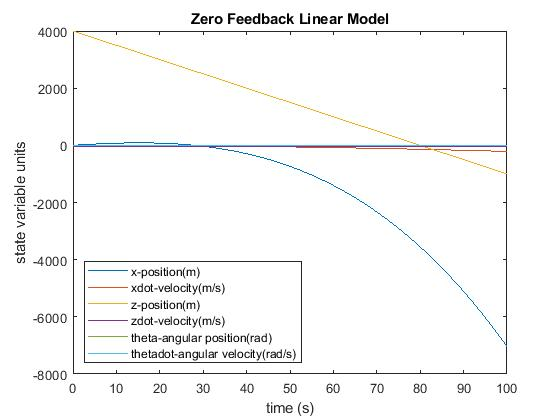
\includegraphics[width=.5\linewidth]{Zeroinput.jpg}
	\caption{Zero Input}
\end{figure}

For this controller, the input vector we use is u = [0;0], which results to no feedback and control. This results to an asymptotically unstable system, that never reaches equilibrium. Figure 1 shows, how the vehicle is falling out of control, and not reaching equilibrium. The vehicles thrusters are stuck at  $F_{le}$ = $F_{re}$ = mg/$\sqrt(2)$, and don't have the ability to change and overcome its initial conditions or gravity.

\subsection{Application of State Feedback}
\begin{figure}[H]
	\centering
	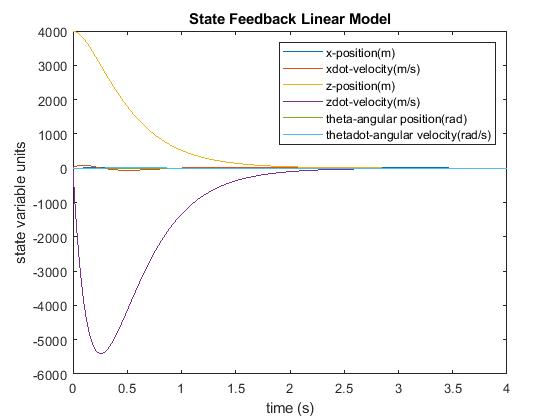
\includegraphics[width=.5\linewidth]{Statefeedback.jpg}
	\caption{State Feedback}
\end{figure}
This controller used the input vector of u=-kx for the vehicle's thrusters. Since the system is meant to reach equilibrium and be asymptotically stable, the k matrix is forced to have 'good' eigenvalues, which in this case were 6 real negative eigenvalues. All values for the state vector converged to zero. Once the vehicle overcame the initial conditions, it moved towards the origin (x = 0, $\theta$ = 0), and hovered at z = 30, with no changes in the velocity ($\dot{x}$, $\dot{z}$, $\dot{\theta}$ =  0). We see figure 2 showing us how the vehicle stabilizes over time to a constant value, at which it hovers. We see that the actuators settle at $F_{le}$ = $F_{re}$ = 2493N. This is only possible as we run it as a linear system, however inputting this controller into a non-linear system would cause it to crash inevitably (shown in figure 6).
\subsection{Examining how the Initial Conditions Affect the Resulting Motion}
\begin{figure}[H]
\centering
\begin{minipage}{.5\textwidth}
	\centering
	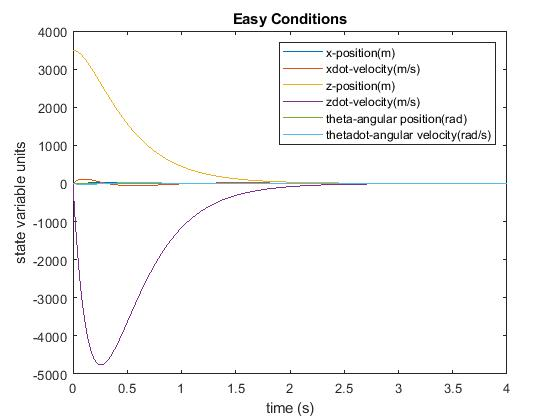
\includegraphics[width=.97\linewidth]{Easyconditions.jpg}
	\caption{Easy Conditions}
	\end{minipage}%
\begin{minipage}{.5\textwidth}
	\centering
	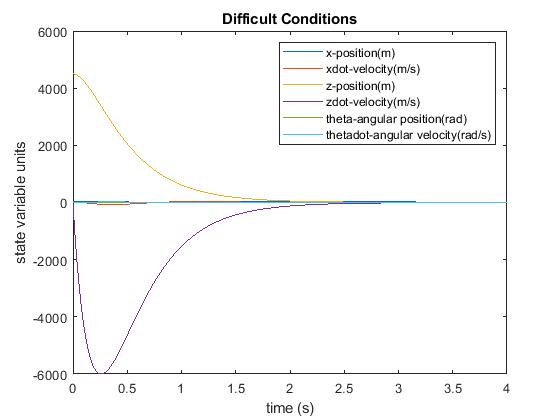
\includegraphics[width=.97\linewidth]{Difficultconditions.jpg}
	\caption{Difficult Conditions}
\end{minipage}
\end{figure}
\begin{figure}[H]
\centering
\begin{minipage}{.5\textwidth}
	\centering
	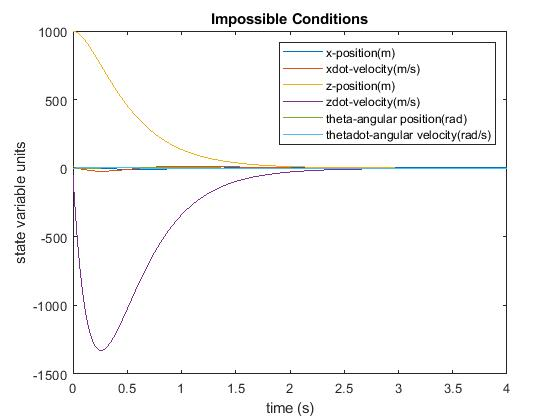
\includegraphics[width=.97\linewidth]{Impossibleconditions.jpg}
	\caption{Easy Conditions}
	\end{minipage}%
\begin{minipage}{.5\textwidth}
	\centering
	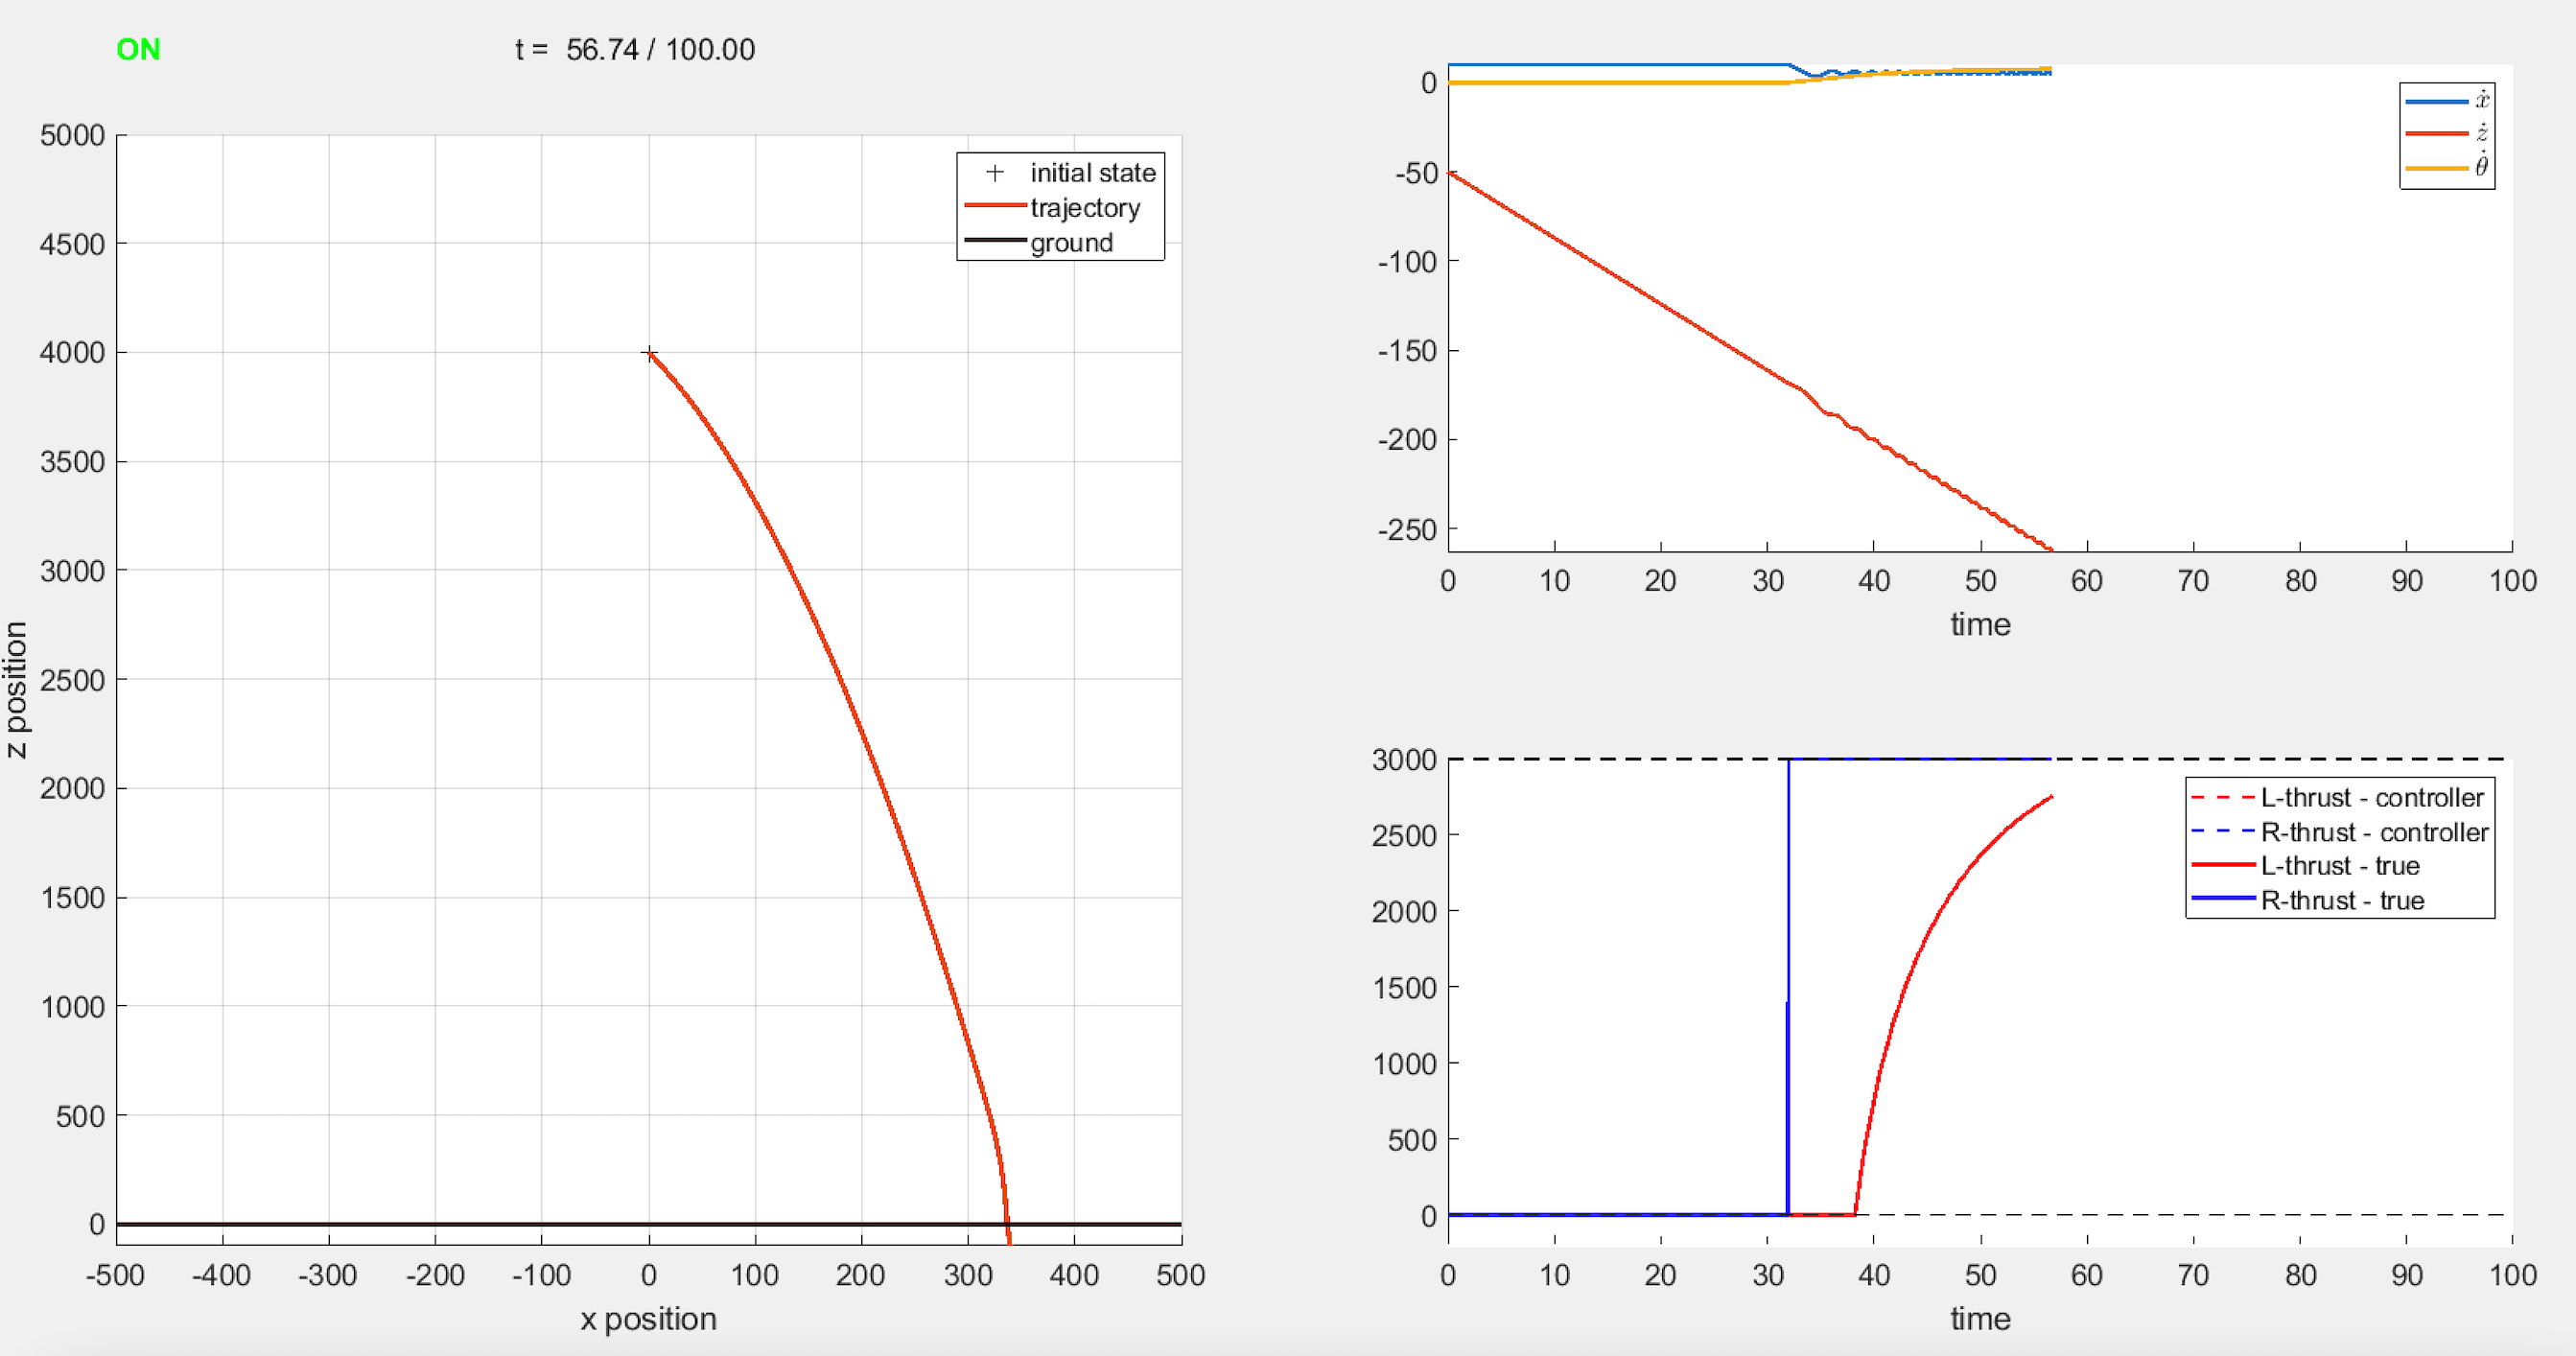
\includegraphics[width=.97\linewidth]{Screen Shot 2020-10-07 at 1.34.13 PM.png}
	\caption{Non-linear System output with a linear system input}
\end{minipage}
\end{figure}
The 3 different conditions used were testing with easy initial conditions [0;0;3500;0;0;0] (shown in figure 3), testing with difficult conditions [40;10;4000;-60;0.1;0.01] (shown in figure 4), and testing with conditions where failure would've been inevitable [0;10;1000;50;0.1;0.01] (shown in figure 5). From the figures shown above, we can see that they converge to zero regardless of the conditions, showing us how it reaches asymptotic stability and equilibrium as they're a linear function. However, if we ran it through the controller output, it would never converge as the designProblem01.m runs it through a non-linear system (Figure 6). Therefore, regardless of the conditions, the linear system will always converge, but will never converge running it in a non-linear system. Thus, this comparison between linear and non-linear system inputs shows the limitations of my controller.
\end{document}